\subsection{Seilzug \hfill IP}
\begin{footnotesize}
    \begin{center}
        \begin{minipage}{0.58\linewidth}
            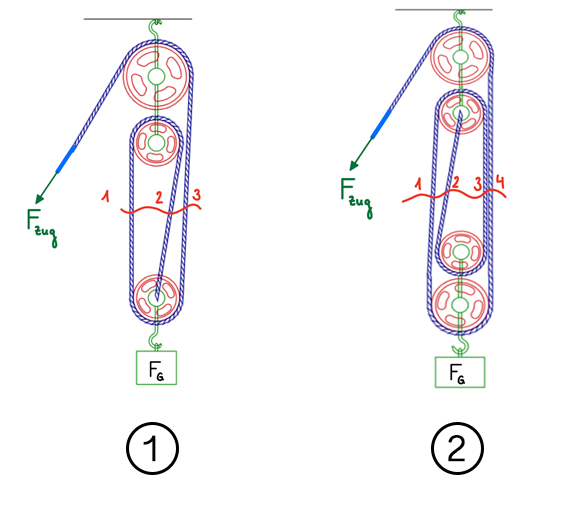
\includegraphics[width = 1.0\linewidth]{MAEIP_Seilzug1}
            \\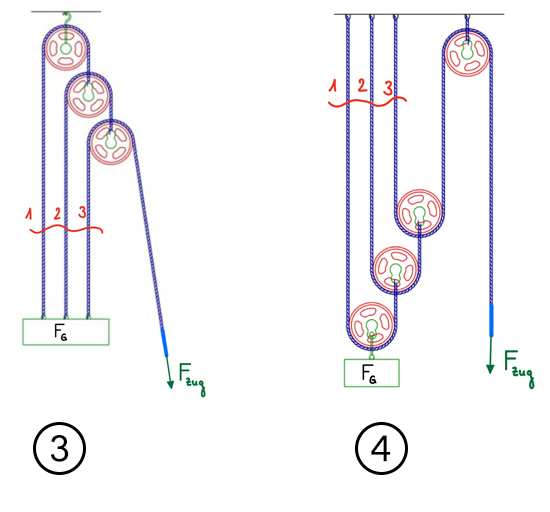
\includegraphics[width = 0.9\linewidth]{MAEIP_Seilzug2}
        \end{minipage}
        \begin{minipage}{0.4\linewidth}
            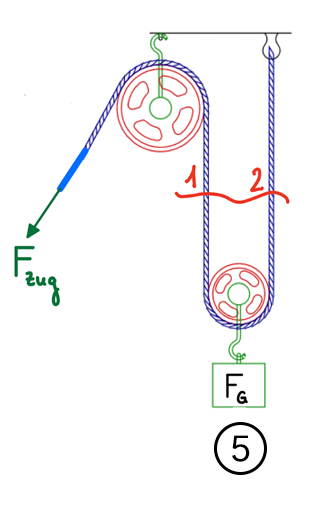
\includegraphics[width = 0.7\linewidth]{MAEIP_Seilzug3}
            \begin{empheq}{align*}
                1. \; \; F_{\text{zug}} &= \frac{1}{3} \cdot F_G 
                \\ 2. \; \; F_{\text{zug}} &= \frac{1}{4} \cdot F_G 
                \\ &= \frac{1}{n} \cdot F_G
                \\ 3. \; \; F_{\text{zug}} &= \frac{1}{7} \cdot F_G 
                \\ 4. \; \; F_{\text{zug}} &= \frac{1}{8} \cdot F_G 
                \\ &= \frac{1}{2^3} \cdot F_G
                \\ 5. \; \; F_{\text{zug}} &= \frac{1}{2} \cdot F_G
            \end{empheq}
        \end{minipage}
    \end{center}
    \begin{empheq}[box=\fbox]{align*}
        \textbf{Wirkungsgrad:  } \eta_F = \eta_R^{\text{\# Rollen}} \quad \mid \quad F_z = \frac{F_g}{\text{\# Rollen}} \cdot \frac{1}{\eta_F}
    \end{empheq}
\end{footnotesize}